\chapter{Tutorial HelloWorld for C}

\section{Scope}

In this tutorial you will learn how to create a model for C from scratch. There are some more steps to do in C compared to Java. The goal is to get familiar with the additional steps. The Java tutorial is a prerequisite for the following explanations. 
You will perform the following steps:

\begin{enumerate}
\item create a new model from scratch for C
\item create structure and behavior similar to Java
\item create a launch configuration for the C code generator
\item setup the C environment
\item generate the source code
\item run the model
\end{enumerate}

Make sure that you have set up the workspace as described in \textit{Setting up the Workspace for C Projects}.


\section{Create a new model from scratch}

Before you can create a new C-model, you have to create a new C project as described in \textit{Setting up the Workspace for C Projects}.
Remember:
\begin{itemize}
\item select the \textit{C/C++} perspective
\item From the main menue select \textit{File->New->C Project}
\item Name the project \textit{HelloWorldC}
\item Project type is \textit{Executable / Empty C Project}
\item Toolchain is \textit{MinGW}
\end{itemize}

The workspace should look like this:

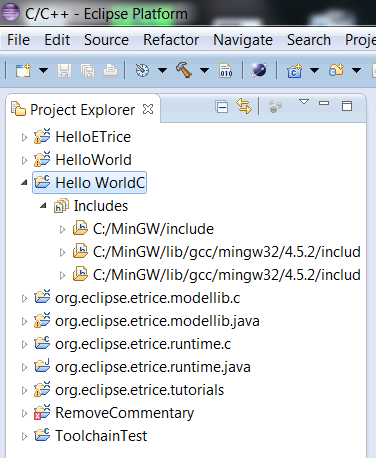
\includegraphics{images/034-HelloWorldC01.png}
% !images/034-HelloWorldC01.png!

The next step is to add the model folder:
Right click on the new project. Select \textit{New->Folder_ and name it _model}.

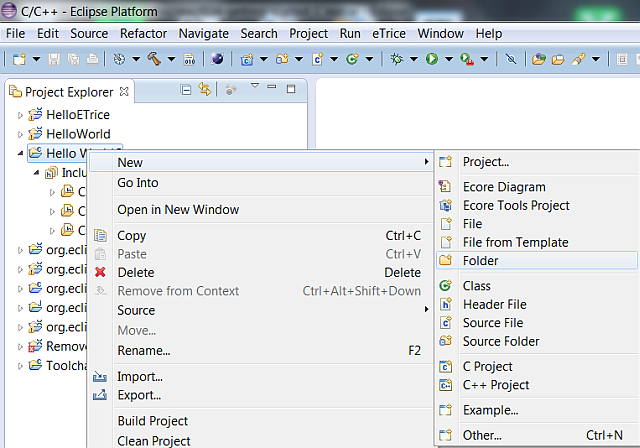
\includegraphics{images/034-HelloWorldC02.png}
% !images/034-HelloWorldC02.png!

Add the model file to the folder. Right click on the new folder. Select \textit{New->file} and name it \textit{HelloWorldC.room}.

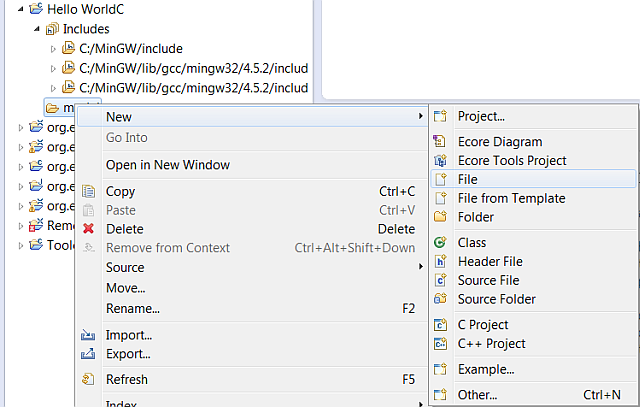
\includegraphics{images/034-HelloWorldC03.png}
% !images/034-HelloWorldC03.png!

Due to the file ending \textit{.room}, the tool will ask you to add the Xtext nature. Answer with \textit{Yes}. 

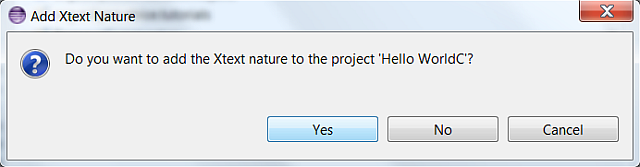
\includegraphics{images/034-HelloWorldC04.png}
% !images/034-HelloWorldC04.png!

The workspace should look like this:

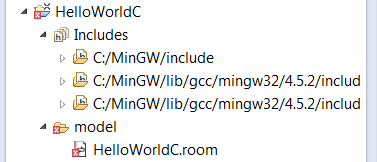
\includegraphics{images/034-HelloWorldC05.png}
% !images/034-HelloWorldC05.png!



\section{Create the HelloWorld model}

Once the model file is created and the Xtext nature is added, you can create the model as you did it for Java.
Creating the model is not the focus of this tutorial. Therefore copy and paste the following code into your model file. Optionally you can open and layout the diagrams.  
Recognize the C specific parts:
\begin{itemize}
\item The action code contains C instead of Java. Later versions will contain a common action language, but for the moment the action language is target specific.
\item The application must be shutdown on model level (see also \textit{etRuntimeConfig.h}).  
\end{itemize}

\begin{verbatim} 
RoomModel HelloWorldCModel {
	import room.basic.types.* from "../../org.eclipse.etrice.modellib.c/model/Types.room"
	SubSystemClass HelloWorldCSubSysClass {
		ActorRef HelloETriceTopRef:AHelloWorldCTop 
	}
	ActorClass AHelloWorldCTop {
		Structure { }
		Behavior {
			StateMachine {
				Transition init: initial -> state0 { }
				State state0 {
					entry {
						"printf(\"HelloWorldC !\\n\");"
						"SubSysClass_shutdown();"
						"\t\t\t\t\t\t"
					}
				}
			}
		}
	}	
}
\end{verbatim}

\section{Create a launch configuration to start the C code generator}

Other than in Java a launch configuration for the C code generator must be created.

From the \textit{Run} menu select \textit{Run Configurations}

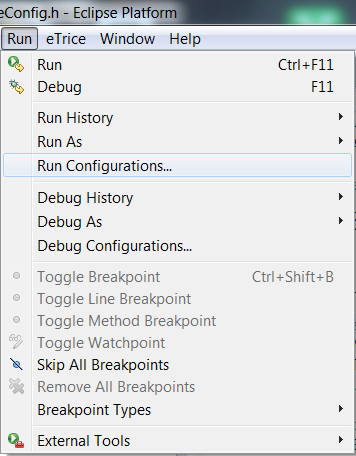
\includegraphics{images/034-HelloWorldC06.png}
% !images/034-HelloWorldC06.png!

Within the dialog select \textit{eTrice C Generator} and click the \textit{New} button to create a new launch configuration.

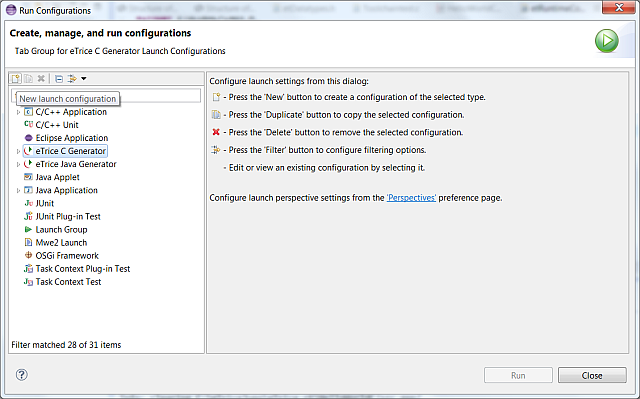
\includegraphics{images/034-HelloWorldC07.png}
% !images/034-HelloWorldC07.png!

A new configuration should be created. Name it \textit{gen\_HelloWorldC} and add the model via one of the \textit{add} buttons.

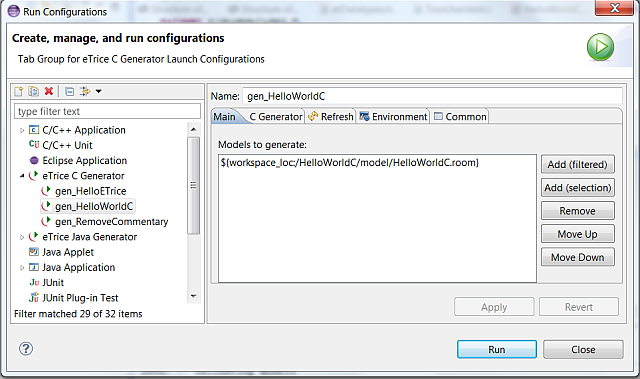
\includegraphics{images/034-HelloWorldC08.png}
% !images/034-HelloWorldC08.png!

In the \textit{Refresh} tab select \textit{The entire workspace} 

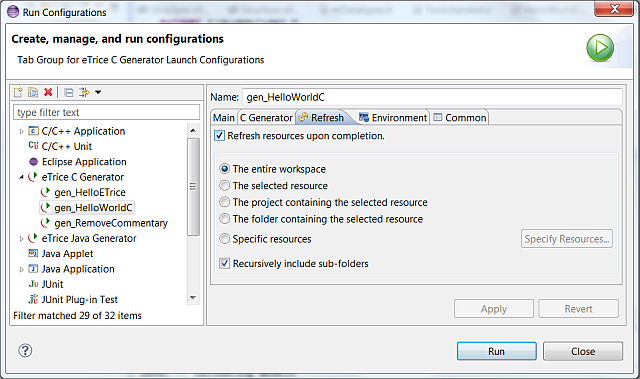
\includegraphics{images/034-HelloWorldC09.png}
% !images/034-HelloWorldC09.png!

In the \textit{Common} tab select \textit{Shared file} and add the \textit{HelloWorldC} project via the \textit{Browse} button.

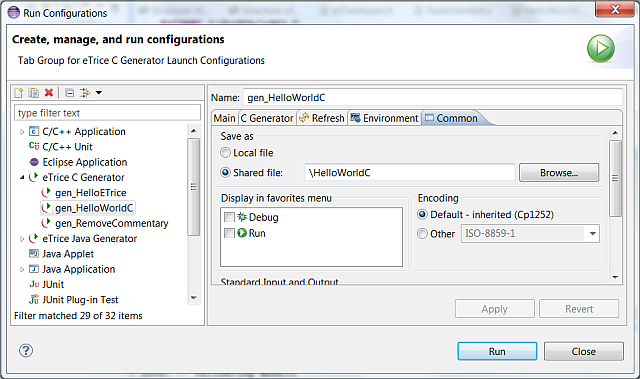
\includegraphics{images/034-HelloWorldC10.png}
% !images/034-HelloWorldC10.png!

Apply your changes. The new configuration should now exist in your workspace.

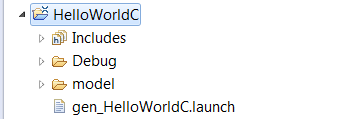
\includegraphics{images/034-HelloWorldC11.png}
% !images/034-HelloWorldC11.png!


\section{Generate the code}

Now you can generate the code as you know it from Java. Right click on the launch configuration and run it as _gen_HelloWorldC_.

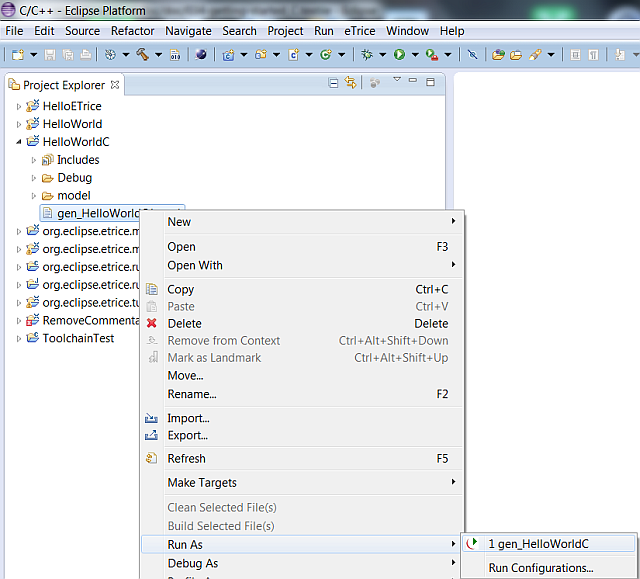
\includegraphics{images/034-HelloWorldC12.png}
% !images/034-HelloWorldC12.png!

The code should be generated.

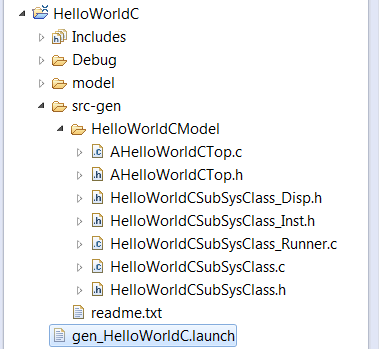
\includegraphics{images/034-HelloWorldC13.png}
% !images/034-HelloWorldC13.png!

\section{Setup the include path}

Before you can build the application you must setup the include path for the runtime system. Right click the project and select \textit{Properties}. Add the include path as described in \textit{setting up the workspace}.

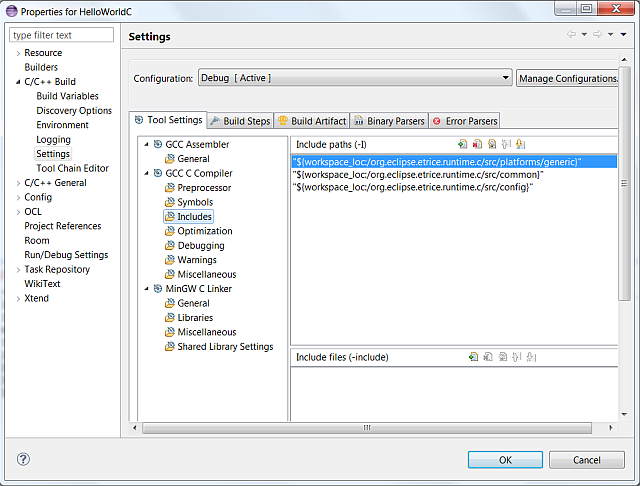
\includegraphics{images/034-HelloWorldC14.png}
% !images/034-HelloWorldC14.png!

Add the runtime library.

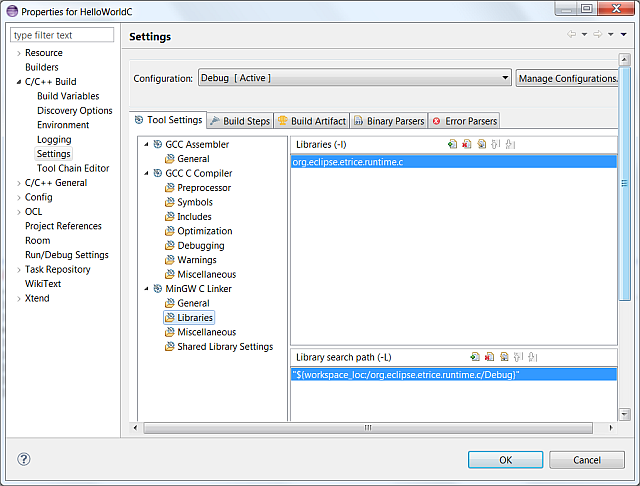
\includegraphics{images/034-HelloWorldC15.png}
% !images/034-HelloWorldC15!

Recognize the name of the library ("org.eclipse.etrice.runtime.c"). The library file on your disk is "liborg.eclipse.etrice.runtime.c.a". 

\section{Build and run the model}

Now you can build the application. Click the build button to build the application.
Run the application as \textit{Local C/C++ Application}.
Verify the output.

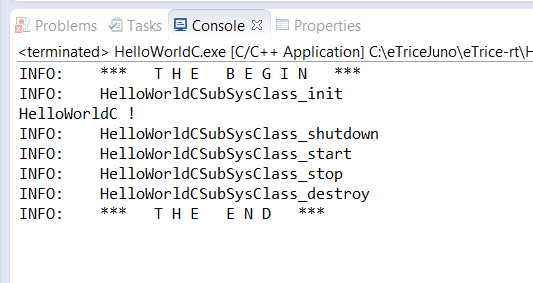
\includegraphics{images/034-HelloWorldC16.png}
% !images/034-HelloWorldC16.png!

\section{Summary}

You are now familiar with all necessary steps to create, build and run an eTrice C model from scratch. You are able to create a launch configuration to start the code generator and to perform all necessary settings to compile and link the application.  

The next tutorial provides an exercise to get more familiar with these working steps.
